\section{Swaps}\label{sec:swaps}
\subsection{The swap graph}
\begin{definition}[arrangement graph, swap graph, swap class]\label{def:swapgraph}
Let $C$ be a finite multiset of labels. The \emph{arrangement graph} $\mathcal G(C)$ has as vertices the distinct arrangements (orderings) of $C$, two being joined if they differ by exchanging two adjacent \emph{distinct} letters. For a source $m$ let $\mathcal A(m)=\{w:K(w)\mid m\}$ be the set of arrangements admissible from $m$. The \emph{swap graph} $\mathrm{Sw}(C,m)$ is the subgraph of $\mathcal G(C)$ induced on $\mathcal A(m)$; its edges are the \emph{legal swaps}, and its components are the \emph{swap classes} of $C$ at $m$. Write $\nu(C,m)$ for their number.
\end{definition}
A vertex of $\mathrm{Sw}(C,m)$ is the history $(m;w)$, and a legal swap is an exchange of adjacent distinct labels of a history that produces an admissible history; the endpoint is unchanged because $m\prod R(N_i)$ does not depend on the order.
\begin{proposition}[the swap graph is an induced subgraph]\label{prop:induced}
The graph on the histories with source $m$ and content $C$, joined by legal swaps, equals $\mathrm{Sw}(C,m)$. In particular two admissible arrangements adjacent in $\mathcal G(C)$ are always joined by a legal swap.
\end{proposition}
\begin{proof}
An edge between two admissible words that differ by an adjacent exchange is, by definition, a legal swap; conversely a legal swap joins two admissible words differing by an adjacent exchange.
\end{proof}
\prov{CW-0345}{D-T7'}{PROVED}{FULL}
\begin{proposition}[numerical commutativity is not admissibility]\label{prop:numcomm}
For all labels $A,B$ the multipliers commute, $R(A)R(B)=R(B)R(A)$, so both orders of $A,B$ have the same endpoint from every source at which both are admissible. Nevertheless the exchange is legal at the state $x$ iff $AB\mid x$ (\cref{prop:diamond}), which is a condition on $x$, not on the multipliers. For instance $(2,3)$ is admissible from $2$ ($2\to9\to48$) while $(3,2)$ is not ($3\nmid2$).
\end{proposition}
\begin{remark}[resemblance to traces and to concurrency]\label{rem:traces}
Adjacent exchanges of commuting letters recall the commutation classes of a trace monoid~\cite{CartierFoata1969,Mazurkiewicz1987,DiekertRozenberg1995}, and the picture of $p$ as a resource of capacity $u_p$ recalls processes with counting semaphores and the directed topology of their state spaces~\cite{Pratt1991,FajstrupEtAl2016}. The resemblance is only that. In a trace monoid independence is a fixed relation on letters; here $A,B$ are interchangeable at $x$ iff $AB\mid x$, which depends on the state, and the classes are not the classes of a congruence on a free monoid. No equivalence with either theory is proved or claimed.
\end{remark}

\subsection{Thresholds of connection; monotonicity}
\begin{theorem}[connection thresholds and the divisibility filtration]\label{thm:paths}
Let $C$ be a multiset and $w,w'$ arrangements of $C$.
\begin{enumerate}[label=(\alph*),itemsep=1pt]
\item $w$ and $w'$ lie in one swap class at the source $m$ iff there is a path $\gamma$ from $w$ to $w'$ in $\mathcal G(C)$ whose threshold $M_\gamma=\lcm_{v\in\gamma}K(v)$ divides $m$. The minimal such $M_\gamma$ form an antichain under divisibility (the \emph{connection thresholds} of the pair).
\item The swap graph depends only on $\mathcal A(m)$. If $m'=\lcm\{K(w):w\in\mathcal A(m)\}$ then $m'\mid m$ and $\mathcal A(m')=\mathcal A(m)$. Hence every swap-graph shape occurring for $C$ occurs at a source in the finite lcm-closure of $\{K(w)\}$, and the classification of $C$ is a finite computation.
\item (\emph{monotonicity}) If $m\mid m^*$ then $\mathcal A(m)\subseteq\mathcal A(m^*)$; the classes at $m^*$ are unions of classes at $m$, together with possibly new classes made of newly admissible arrangements. A class never splits, but $\nu(C,m)$ is not monotone in $m$.
\end{enumerate}
\end{theorem}
\begin{proof}
(a) A path has all its vertices admissible iff every $K(v)$, $v\in\gamma$, divides $m$, iff their lcm does; and a minimal set of thresholds is an antichain by definition. (b) $m'$ divides $m$ since each $K(w)$ with $w\in\mathcal A(m)$ does; $\mathcal A(m')\supseteq\mathcal A(m)$ since those $K(w)$ divide $m'$, and $\mathcal A(m')\subseteq\mathcal A(m)$ because $m'\mid m$. (c) $K(w)\mid m\mid m^*$. For non-monotonicity see the examples below.
\end{proof}
\prov{CW-0346}{D-T8}{PROVED}{FULL}
\begin{example}[class counts are not monotone]\label{ex:nonmono}
For $C=\{2,3,14\}$: $\nu=2$ at $m=14$ and $\nu=1$ at $m=28$ (\cref{thm:2314}). For $C=\{2,3,8\}$ the thresholds are $K(2,3,8)=2$, $K(3,2,8)=K(3,8,2)=3$, $K(8,3,2)=8$, $K(2,8,3)=K(8,2,3)=16$ and one finds $\nu=1,2,1$ at the sources $2,8,16$, which are totally ordered by divisibility: a class count can rise and fall along a divisibility chain.
\end{example}

\subsection{Same content, different swap classes: the source-\texorpdfstring{$14$}{14} example}
\begin{example}[source $14$]\label{ex:src14}
From the source $14$ the content $\{2,3,14\}$ has exactly two admissible arrangements (\cref{ex:K}):
\[
 14\xrightarrow{14}225\xrightarrow{3}1200\xrightarrow{2}5400,\qquad
 14\xrightarrow{2}63\xrightarrow{3}336\xrightarrow{14}5400 .
\]
They have the same source, the same content and the same endpoint $5400$, and neither has a legal swap: exchanging $(14,3)$ at the state $14$ needs $42\mid14$; $(3,2)$ at $225$ needs $6\mid225$; $(2,3)$ at $14$ needs $6\mid14$; and $(3,14)$ at $63$ needs $42\mid63$ --- all four fail by \cref{prop:diamond}(c). The mechanism is resource contention: the prime $2$ has capacity $1$ at $14$; both $2$ and $14$ consume it and only the label $3$ (with $4=3+1$) produces it, so exactly one of $\{2,14\}$ can run before $3$. The two histories also have different fibre sequences and different occurrence events (\cref{sec:events}).
\end{example}
\begin{figure}[tbp]\centering
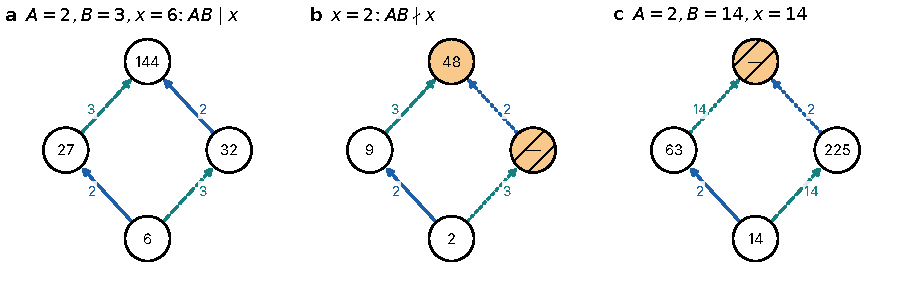
\includegraphics[width=\textwidth]{fig07_swap_diamonds}
\caption{\textbf{Legal and forbidden swap diamonds (exact).} Each panel shows the states (circles) reached from a state $x$ by the labels $A$ (solid blue edges) and $B$ (dashed teal edges); dotted edges and hatched orange nodes are inadmissible. (a) $A=2$, $B=3$, $x=6$: $AB\mid x$, the diamond closes at $144$. (b) $x=2$: $A=2$ is admissible but $B=3$ is not, so only one side exists. (c) $A=2$, $B=14$, $x=14$: both labels are admissible at $14$ but $AB=28\nmid14$, so after $2$ the label $14$ fails ($63$ is not divisible by $14$) and after $14$ the label $2$ fails. Theorem illustrated: \cref{prop:diamond}.}\label{fig:diamonds}
\end{figure}
\noindent The figure above is \cref{fig:diamonds}; its caption states the exactness of what is drawn.
\begin{theorem}[complete classification of $\{2,3,14\}$]\label{thm:2314}
The thresholds are $K=14$ for $(14,3,2),(2,3,14)$, $K=28$ for $(14,2,3),(2,14,3)$, and $K=21$ for $(3,14,2),(3,2,14)$. The number of swap classes of $\{2,3,14\}$ at the source $m$ is
\[
 \nu=\begin{cases}0&\text{if neither }14\text{ nor }21\text{ divides }m,\\ 2&\text{if }14\mid m\text{ and }\gcd(m/14,6)=1,\\ 1&\text{otherwise.}\end{cases}
\]
In particular, the two arrangements $(14,3,2)$ and $(2,3,14)$ lie in one class iff $28\mid m$ or $42\mid m$ (their connection thresholds), and from $m=14q$ there are two classes iff $\gcd(q,6)=1$. All admissible arrangements from $m$ end at $m\cdot2700/7$.
\end{theorem}
\begin{proof}
The thresholds were computed in \cref{ex:K}. Order the arrangements around the hexagon $\mathcal G(C)$ as $\sigma_0=(14,3,2)$, $\sigma_1=(3,14,2)$, $\sigma_2=(3,2,14)$, $\sigma_3=(2,3,14)$, $\sigma_4=(2,14,3)$, $\sigma_5=(14,2,3)$ (consecutive ones, and $\sigma_5,\sigma_0$, differ by an adjacent exchange). Then $\sigma_0,\sigma_3$ have threshold $14$ and are antipodal, $\sigma_1,\sigma_2$ have threshold $21$ and are adjacent, and $\sigma_4,\sigma_5$ have threshold $28$ and are adjacent. Every threshold is a multiple of $7$, so $7\mid m$ is necessary for any arrangement to be admissible. Now $\mathcal A(m)$ is the union of the pairs whose threshold divides $m$. If $14\nmid m$ then $28\nmid m$ and $\mathcal A(m)\subseteq\{\sigma_1,\sigma_2\}$, which is empty if $21\nmid m$ and one edge (one class) if $21\mid m$. If $14\mid m$ then $\sigma_0,\sigma_3\in\mathcal A(m)$; adding the $28$-pair when $28\mid m$ gives the path $\sigma_3\sigma_4\sigma_5\sigma_0$, adding the $21$-pair when $21\mid m$ gives the path $\sigma_0\sigma_1\sigma_2\sigma_3$; in either case the graph is connected, while with neither it is two isolated vertices. Finally $14\mid m$ and $21\nmid m$ and $28\nmid m$ means $14\mid m$, $3\nmid m$ and $m/14$ odd, i.e.\ $\gcd(m/14,6)=1$. The connection thresholds are $\lcm(14,28)=28$ and $\lcm(14,21)=42$. The common endpoint is $mR(2)R(3)R(14)=m\cdot\frac92\cdot\frac{16}3\cdot\frac{225}{14}=m\cdot\frac{2700}7$.
\end{proof}
\prov{CW-0348}{D-T10}{PROVED}{FULL}
\begin{corollary}[an infinite family of complete histories]\label{cor:family14}
Let $q\ge1$ be squarefree and coprime to $42$. Then $14q$ is squarefree, and the two complete histories $(14q;14,3,2)$ and $(14q;2,3,14)$, both ending at $5400q$, lie in different swap classes.
\end{corollary}
\begin{proof}
$14q$ is squarefree because $q$ is squarefree and coprime to $2\cdot7$; $\gcd(q,6)=1$ gives two classes by \cref{thm:2314}.
\end{proof}
\prov{CW-0342}{D-T5}{PROVED}{FULL}
\begin{figure}[tbp]\centering
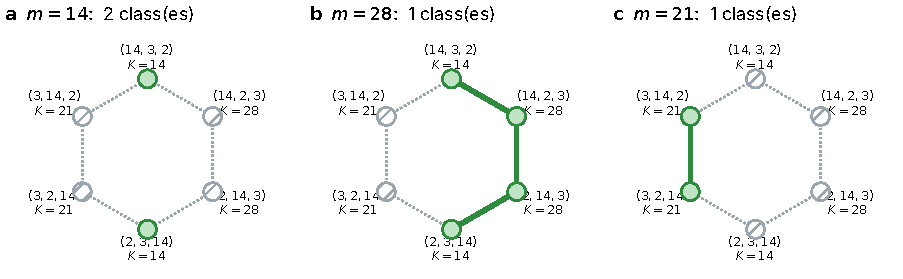
\includegraphics[width=\textwidth]{fig08_same_content_two_components}
\caption{\textbf{The same content in different swap components (exact).} The hexagon $\mathcal G(\{2,3,14\})$ with the threshold $K$ of each arrangement; admissible vertices at the source $m$ are shaded green and joined by thick solid green lines, inadmissible ones are hatched. (a) $m=14$: the antipodal pair $(14,3,2),(2,3,14)$, two classes, with the histories of \cref{ex:src14}. (b) $m=28$: the $28$-pair joins them, one class. (c) $m=21$: only the $21$-pair, one class. Theorem illustrated: \cref{thm:2314}.}\label{fig:hex}
\end{figure}
\noindent The figure above is \cref{fig:hex}; its caption states the exactness of what is drawn.
\begin{remark}
\Cref{thm:2314} relaxes a restriction of the earliest release: there the pair was shown for $q$ squarefree and coprime to $210$; the condition on the prime $5$ is unnecessary for the statement about fixed-source histories, as the proof shows (and $7\nmid q$ is needed only for squarefreeness of the source).
\end{remark}
